\scanpage{54}
\mspage{53}

First, we shall isolate the axioms for $\leq$

\uline{$\mathcal C$ 1} a) $\mathcal F\ne\varnothing$

\deleted{\uline{\unsure{C 2}}} b) If $F\in\mathcal F_{\leq}$, and $(F_i)_{i\in I}$ is a family of objects of $\mathcal F$ with $F_i\leq F$, then $\underset{i}{\mathrm{Sup}}\,F_j$ exists. (Every family of figures bounded above has a least upper bound.)\figure{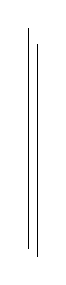
\begin{tikzpicture}\draw (0,0)--(0,2.8);\draw (.12,-.1)--(.12,2.6);\end{tikzpicture}}

\uline{Corollary} $\mathcal F$ has a least ele\deleted{\unsure{ment|ment}} (namely, the $\mathrm{Sup}$ of the empty family of objects)

\uline{NB} In the presence of \deleted{\unsure{C2}} \uline{C 1 b)}, the validity of a) \uline{is equivalent} to that of the corollary.

The least \unsure{element|element} is called the \uline{empty figure}, denoted $\varnothing_{\mathcal F}$ or simply $\varnothing$, by abuse of language, and if confusion is not to be feared

\figure{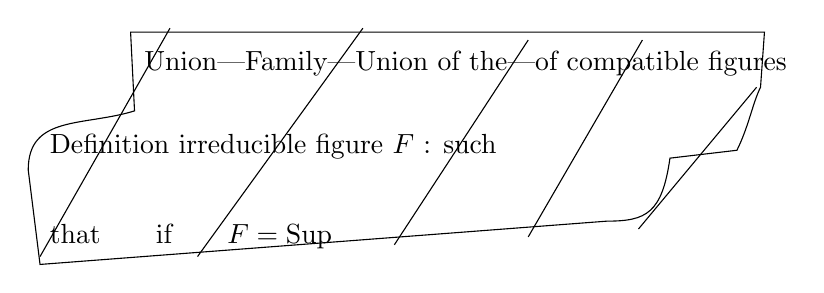
\begin{tikzpicture}[x=1cm,y=1cm]
\node[anchor=west] at (1.2,2.2) {\deleted{\unsure{Union|Family|Union} \unsure{of the|of} compatible figures}};
\node[anchor=west] at (0,1.15) {\deleted{\uline{Definition} \uline{irreducible} \uline{figure $F$ : such}}};
\node[anchor=west] at (0,0) {\deleted{that\qquad if\qquad $F=\mathrm{Sup}$}};
\draw (1.15,2.6)--(9.2,2.6)--(9.15,1.9) .. controls (9.05,1.7) and (9.0,1.4) .. (8.85,1.1) -- (8.0,1.0) .. controls (7.9,.3) and (7.7,.2) .. (7.2,.2) -- (0,-.35)--(-.15,.85) .. controls (-.15,1.55) and (.55,1.4) .. (1.2,1.6)--cycle;
\draw (0,-.25)--(1.65,2.65) (2.0,-.25)--(4.1,2.65) (4.5,-.1)--(6.2,2.5) (6.2,0)--(7.65,2.5) (7.6,.1)--(9.1,1.9);
\end{tikzpicture}}

\uline{Compatible} figures, set of \deleted{\unsure{compatible}} compatible figures : \deleted{\unsure{one which|which}} \inserted{as a whole} (or \uline{configuration}) : which is bounded above for $\leq$. \margin{P} Generated figure, or \uline{union} ($F\vee G$, $\bigvee_i f_i$, $\mathrm{Sup}\,F_i$, sometimes denoted $F\cup G$ \unsure{or|--} $\deleted{F}\bigcup_iF_i$ cf below).

\uline{Definition} \uline{Irreducible figure} $F$ : such that $\displaystyle F=\underset{i\in I}{\mathrm{Sup}}\,F_i\ \overset{-}{\Longrightarrow}\ \exists i\in I,\ F_i=F$.

\deleted{\uline{C 2}} Irreducible figures are called \uline{multistrata}. \inserted{The set of multistrata denoted $ M$} Irreducible figures
